%
% File acl2014.tex
%
% Contact: koller@ling.uni-potsdam.de, yusuke@nii.ac.jp
%%
%% Based on the style files for ACL-2013, which were, in turn,
%% Based on the style files for ACL-2012, which were, in turn,
%% based on the style files for ACL-2011, which were, in turn, 
%% based on the style files for ACL-2010, which were, in turn, 
%% based on the style files for ACL-IJCNLP-2009, which were, in turn,
%% based on the style files for EACL-2009 and IJCNLP-2008...

%% Based on the style files for EACL 2006 by 
%%e.agirre@ehu.es or Sergi.Balari@uab.es
%% and that of ACL 08 by Joakim Nivre and Noah Smith

\documentclass[11pt]{article}
\usepackage{acl2014}
\usepackage{times}
\usepackage{url}
\usepackage{latexsym}
\usepackage{float}
\usepackage{graphicx}
\usepackage[inline]{enumitem}
\usepackage[linewidth=1pt]{mdframed}
\usepackage{lipsum}


%\setlength\titlebox{5cm}

% You can expand the titlebox if you need extra space
% to show all the authors. Please do not make the titlebox
% smaller than 5cm (the original size); we will check this
% in the camera-ready version and ask you to change it back.


\title{Extracting contingent event pairs in  blog corpus}

\author{Abhinav Venkataraman  \\
  {\tt abhinav@soe.ucsc.edu} \\\And
  Keshav Mathur \\
  {\tt kemathur@ucsc.edu} \\}

\date{}

\begin{document}
\maketitle
\begin{abstract}
We implement and evaluate different unsupervised methods for learning event pairs that are likely to be
\texttt{CONTINGENT} on one another\cite{film}. We build language model based on SRILM toolkit rather than pure Manshadi's approach. We compare and contrast different techniques for those data whose temporal coherence are yet to be proved. We would evaluate these models using MTurks, Narrative Cloze and a novel and unique Discriminative method.
\end{abstract}


\section{Introduction}
Any narrative story can be seen as a chain of ordered set of events. In this project, we would like to focus on extracting the event pairs which are contingent on each other, in an unsupervised data driven fashion. It would be nice to try to understand more about the internal structure of the different types of stories, basically to find out what kinds of action sequences characterize them. Extracting contingent events is a prerequisite in many NLP tasks like text coherence, entailment, question answering and information retrieval(giriju).Previous work shows good results in finding the contingent event pairs from film scenes by modeling the likelihood between events[chao]. \\
\medskip \\
We feel trying to extract such causal chains from personal stories may provide for better common sense reasoning and help in script learning in common scenarios about which people often blog. Also trying out different event representations could help yield better understanding of which components contribute to the discovery of the \texttt{CONTINGENT} relation between events. 

\section{Related Works}
Giru et al. focussed on giving a statistical measure to the events that are in causal relationship by defining causal potential\cite{cp}. Chambers et al. defined such events with causal relationships as narrative event chains and came out with different ways of learning\cite{nec}. They also build a new method of identifying event semantics that jointly learns event relations and their participants from unlabeled corpora\cite{cloze}. Chiacros solved the same problem by providing a method for identifying a discource connective between different utterences in text\cite{chiacro}. Manshadi et al. tried to solve a similar problem by  learning a probabilistic model of event sequences using statistical language modeling techniques\cite{manshadi}. Quang Xuan Do et al. followed Chiacros methodology of solving similar problem by feeding discourse connectives and the particular discourse relation in addition to the distirbutional similarity to identify causal relations between events\cite{do} \\
\smallskip \\
Our hypothesis and methodology is completely based from Chao et al.\cite{film} by creating the same event representation and evaluate some of the methodologies done by others which are mentioned above and see how they perform for sports and travel stories. We believe that the underlying assumption of temporal coherence do exist in the sports and travel stories.  


\section{Methods}
In this project we want to test different measures of contingency and event representations to extract contingent event pairs from the corpus and try to compare and contrast them. An event can be represented in many forms. The ones we want to test out are:
\begin{enumerate*}[label=\itshape\alph*\upshape)]
\item Just the verb
\item Verb + Subject+Object
\item Verb + Subject
\item Verb + Object
\item Multi-argument event representation as stated by Mooney \cite{mooney}
\end{enumerate*}    

For each of these representations we will calculate three different measures of contingency used in previous works: \\
\smallskip \\

{\bf Point wise Mutual Information.} It is a symmetric measure of two events occurring adjacent to each other in a document. So this finds the probabilities of two events appearing close to one another but not actually imply causality\cite{nec,cloze}. \\
The PMI between two events is defined as: 
\begin{equation}\label{pmi}
pmi(e_1,e_2) = \log\frac{P(e_1,e_2}{P(e_1)P(e_2)}
\end{equation}
in which $e_1$, $e_2$ are two events. $P(e_1)$ is the probability that event $e_1$ occur in corpus : 
\begin{equation}
P(e_1) = \frac{count(e_1)}{\Sigma_x count(e_x)}
\end{equation}
The joint probability of both events occuring together($P(e_1,e_2)$) is given by :
\begin{equation}
P(e_1,e_2) = \frac{count(e_1)}{\Sigma_x \Sigma_y count(e_x,e_y)}
\end{equation}
\smallskip \\

{\bf Causal Potential.} A more refined measure for causality was proposed by \cite{cp}. They define a manipulation test for annotators trying to judge if event A caused event B. 
\begin{enumerate}
\item[(i)] Does event A occur before (or simultaneously) with event B?
\item[(ii)]  Keeping constant as many other states of affairs of the world in the given text context as possible, does modifying event A entail predictably modifying event B?
\end{enumerate}
Answering yes to both these questions would imply causality.  \\
\textbf{CP} is thus defined as :
\begin{equation}
\phi(e_1,e_2) = pmi(e_1,e_2) + \log\frac{P(e_1 \rightarrow e_2)}{ P(e_2 \rightarrow e_1)} 
\end{equation}
where $pmi(e_1,e_2)$ is given by (\ref{pmi}). \\
\smallskip \\
PMI and Causal Potential are found for events adjacent in a document. We plan to define adjacency as a 2-skip model. If a document is represented as a series of events. $e_1, e_2, e_3, e_4$ and $e_5$ then the ordered pairs for which the counts will be generated are: $(e_1,e_2), (e_1,e_3), (e_1,e_4), (e_2,e_3), (e_2,e_4),$  $(e_2,e_5), (e_3,e_4), (e_3,e_5), (e_4,e_5)$. \\
The event pairs rated highly on these measures will be used for the different evaluation experiments that we define in the coming section. \\
\smallskip \\
{\bf Probabilistic Language Models.}
We build a statistical language model using the verbs alone where we represent each document as a sequence of verbs \cite{manshadi}. 
We compute the bigram probabilities of verbs that occur in the document and it is defined as :
\begin{equation}
P(w_1,w_2) = \frac{count(w_1,w_2)}{count(w_1)}
\end{equation}
\smallskip \\
So for an example document:
\begin{quote}
\textit{John Doe opened the box. He ate the chocolates.}
\end{quote}
 This sentence is converted to “\texttt{open,ate}”. Using this sequence of verbs we calculate bigram probabilities which might imply contingency between the events. \\
\smallskip \\
\subsection{Difficulties to be faced}
In future we anticipate few difficulties that are to be faced in our methodologies. They are : 
\begin{itemize}
\item  We are trying to use the SRILM toolkit for getting the necessary counts and probabilities for each of these measures. It is going to be really straight forward for building the bigram language model but non-trivial for getting the statistics for PMI and CP as there events are considered over a 2-skip model and we don’t yet know how to incorporate that into SRILM. If not possible we will be writing code for for finding the counts and the necessary probabilities.
\item The data we have may not not be sufficient for finding the necessary statistics and we may have to annotate more.
\item The representation used in \cite{mooney} may prove to be complicated and time consuming to implement.
\end{itemize}
 
\section{Data}
A sample story from our corpus looks like this :
\begin{mdframed}
\small This morning my dad, uncle and I went for a short hike around the Short Hill. I had long known that part of the mountain was part of Harpers Ferry National Park, but only last week discovered access to the site . I told my dad about it and he was interested to check it out. Despite the cold drizzley weather we set out, being careful to not injure our selfs stepping into deep piles of leaves as I had the last time I visited the site. Almost immediately we encountered the ruins of an old lime kiln, which sadly I neglected to take a picture. A little further up the trail we came to the ruins of the old River Mill. We then made our way around the Short Hill on an old road bed, catching good views across and up river. That last pic was taken from a 60ft bluff above the river, and though you can't make it out in the picture, good views of Harpers Ferry 5 miles distant were had. Though the hike was short and we only stuck to the shore and did not attempt the mountain it was enjoyable and left me impatient for the spring when i can mount a full expedition of the area. Definitely going to need a machete because the undergrowth is going to be bad, good shoes and a hiking stick will also be necessary on the steep ungraded slopes. Check out my facebook for a few pics from the hike. 
\end{mdframed} 
\vspace{2em}
The data we are using consists of a number of stories divided into two major domains: travel and sports. These stories were taken from The Internet Personal Story Archive\cite{ipsa} which is a collection of blog posts taken from the internet. Stories within each domain are also sub categorized into a number of fine grained topics like hiking, skiing, scuba diving etc. for travel and cricket, soccer , swimming for sports. At present we have 440 stories for travel blogs and 280 for sports. We have considered 67 stories of travel as our held out test set and built the bigram model on 357 stories. Similarly for sports, 238 for building the language model and 42 for testing. After running the initial experiments on this corpus we will assess if there is a need for more data and if need be, annotate more data into each category. \\
\smallskip \\
We use Stanford CoreNLP\cite{corenlp} toolkit to get the annotations. We feed into the parser the entire corpus of stories and yield corresponding XML files which contain necessary annotations. We parse the XML output to get the verbs in their lemmatized form, which are actions and also extract the subject and object of the verb from the dependency parse. We are trying to use the SRILM toolkit for getting the necessary counts and probabilities for each of these measures\cite{srilm}.

\section{Evaluation}
We have three evaluations in mind :
\subsection{MTurks}
We have planned to set up three HITs where each task would have involving the presence and absence of arguments for events and also ordering of events whether it matters or not.  We plan to more or less replicate the set up that was mentioned in \cite{film}. Each HIT would have the task for which the annotator needs to say whether the events given would occur together or not. The same objective is done with order maintained and also done with no preference on the order of events.  The other HIT task would to present event with arguments and ask the annotators how likely would given set of events occur together. Sample piece of a format of turk job is given in the picture below.\footnote{Obtained from \cite{film} paper  } \\

\begin{figure}[H]
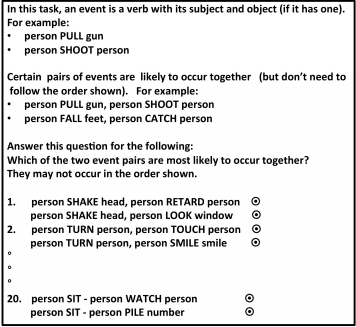
\includegraphics[scale=0.65]{turk.png}
\end{figure}


\subsection{Cloze Task}
One event is removed from a narrative sequence and the task for a model is to predict the missing event , its and typed dependency.  We plan to implement this to evaluate our models and see how well it performs \cite{nec}.
\subsection{Discriminative Task}
The third task that we plan to use for evaluation is the discriminative task. In this task we generate a random permutation of the events of a document and see if the models assign a higher probability to the random permutations or the original ordering of events.
To our knowledge this task hasn’t been used much for the kind of problem we are tackling. So it will be a good experiment to see how these models perform. \\ 
\smallskip \\

\section{Schedules and Responsibilities}
\subsection{Milestones Achieved}
We have successfully built the language models for both categories sports and travel. We represented each document as a sentence of verbs and fed each category into the SRILM toolkit which gave out the bigram model. We then computed the preplexity score for each of them on kndiscount smoothening after discounting the words and here goes the results: \\
\underline{\textbf{Results of Bigram Model}} \\
\begin{table}[H]
\begin{center}
\begin{tabular}{|c|c|}
\hline 
\bf Test & \bf  Preplexity \\ 
\hline 
Travel LM on Travel & 87.497 \\ 
\hline 
Travel LM on Sports & 152.325 \\ 
\hline 
Sports LM on Sports & 117.409 \\
\hline
Sports LM on Travel & 105.323 \\
\hline
\end{tabular} 
\end{center}
\end{table}

\underline{\textbf{Results of Trigram Model}} \\
\begin{table}[H]
\begin{center}
\begin{tabular}{|c|c|}
\hline 
\bf Test & \bf  Preplexity \\ 
\hline 
Travel LM on Travel & 92.6553 \\ 
\hline 
Travel LM on Sports & 154.198 \\ 
\hline 
Sports LM on Sports & 121.555 \\
\hline
Sports LM on Travel & 110.959 \\
\hline
\end{tabular} 
\end{center}
\end{table}
Travel LM on Travel means language model built on travel data was tested on travel's test data. Similarly, Travel LM on Sports means the language model built on travel data was tested on sports. Perplexity can be defined as the as the number of guesses you need to make about the next word/verb/event given the context. Therefore, lower the perplexity score, the higher the coherence.It is to be noted that Sports LM on Travel yields lower perplexity in both cases which means Sports LM is not that coherent when compared to travel as Travel LM on sports yields greater perplexity than Travel LM on travel. \\
In order to accomplish this task the work was split accordingly which is given below:  \\
\smallskip \\
{\bf Keshav}:  
\begin{itemize}
\item Processed the stories using the Stanford CoreNLP pipeline.
\item Wrote parsers for the XML output given by StanfordCoreNLP in python.
\item Created the text input for the SRILM toolkit in which each line represents all the verbs in a document.
\end{itemize} 
\smallskip
{\bf Abhinav :} 
\begin{itemize}
\item Set up the SRILM toolkit
\item Compute the verb pair counts for the corpus.
\item Built various language models with and without smoothening for bigrams and trigrams.
\item Find the perplexity scores.
\end{itemize} 
\subsection{Timeline for Future}
Although our next steps are evidently explained before, the timeline for the future are : \\
{\bf Keshav: }
\begin{itemize}
\item Get the statistics for the Verb + Object representation and the Verb + Object + Subject representation.
\item Perform the experiments for the discriminative task.
\end{itemize}
\smallskip
{\bf Abhinav: }
\begin{itemize}
\item Get the statistics for the Subject + Verb representation
\item Perform the experiments for the cloze task and set up the HITs on Mechanical turk.
\end{itemize}
Both of us would work together on mooney's event representation and build the models as discussed in methods section for that representation 
%\begin{table}[h]
%\begin{center}
%\begin{tabular}{||c|cl|}
%\hline \bf Test & \bf Perplexity  \\ 
%Travel LM on travel & 15 pt \\
%\hline
%\end{tabular}
%\end{center}
%
%\end{table}





% include your own bib file like this:
%\bibliographystyle{acl}
%\bibliography{acl2014}

\begin{thebibliography}{}

\bibitem[\protect\citename{Girju and Brandon}2009]{cp}
Beamer, Brandon, and Roxana Girju,.
\newblock 2009.
\newblock {\em Using a bigram event model to predict causal potential}, 
\newblock Computational Linguistics and Intelligent Text Processing
\newblock Springer Berlin Heidelberg, 2009. 430-441

	   
\bibitem[\protect\citename{Chambers and Jurafsky}2008]{nec}
	Chambers, Nathanael, and Daniel Jurafsky,
	\newblock 2008.
	\newblock{\em Unsupervised Learning of Narrative Event Chains. }
	  ACL. Vol. 94305.

\bibitem[\protect\citename{Chambers and Jurafsky}2009]{cloze}
	Chambers, Nathanael, and Dan Jurafsky,
	\newblock 2009
	\newblock{\em Unsupervised learning of narrative schemas and their participants}
	\newblock In Proceedings of the Joint Conference of the 47th Annual Meeting of the ACL and the 4th International Joint Conference on Natural Language Processing of the AFNLP
	  \newblock Volume 2-Volume 2, pp. 602-610,Association for Computational Linguistics

\bibitem[\protect\citename{Chiarcos} 2012]{chiacro}
	Chiarcos, Christian.,
	\newblock 2012,
	\newblock{\em Towards the unsupervised acquisition of discourse relations},
	\newblock  Proceedings of the 50th Annual Meeting of the Association for Computational Linguistics: Short Papers-Volume 2,
	\newblock Association for Computational Linguistics.

	
\bibitem[\protect\citename{Manshadi et al.}2008]{manshadi}
	Manshadi, Mehdi, Reid Swanson, and Andrew S. Gordon,
	\newblock 2008,
	\newblock{\em Learning a Probabilistic Model of Event Sequences from Internet Weblog Stories},
	 \newblock FLAIRS Conference. 2008.

\bibitem[\protect\citename{Do et al.}2011]{do}
	Do, Quang Xuan, Yee Seng Chan, and Dan Roth.
	\newblock 2011,
	\newblock{\em Minimally supervised event causality identification},
	 \newblock Proceedings of the Conference on Empirical Methods in Natural Language Processing. 
	 \newblock Association for Computational Linguistics.
	 
\bibitem[\protect\citename{Chao et al.}2013]{film}
	Hu, Zhichao and Rahimtoroghi, Elahe and Munishkina, Larissa and Swanson, Reid and Walker, Marilyn A.,,
	\newblock  October, 2013.
	\newblock{\em Unsupervised Induction of Contingent Event Pairs from Film Scenes.}
	\newblock In Conference on Empirical Methods in Natural Language Processing,
	\newblock Seattle, WA
	 
\bibitem[\protect\citename{Pichotta and Mooney}2014]{mooney}
	Pichotta, Karl, and Raymond J. Mooney.
	\newblock 2014.
	 \newblock{\em Statistical script learning with multi-argument events}
	 \newblock EACL(2014), 220.
	  

\bibitem[\protect\citename{Reid}]{ipsa}
  	Reid Swanson,
  	\newblock {\em The Internet Personal Story Archive}.
  	\newblock reid@reidswanson.com.
  
\bibitem[\protect\citename{Manning et al.}2014]{corenlp}
	Manning, Christopher D. and  Surdeanu, Mihai  and  Bauer, John  and  Finkel, Jenny  and  Bethard, Steven J. and  McClosky, David,
	\newblock June 2014.
	\newblock{\em The {Stanford} {CoreNLP} Natural Language Processing Toolkit},
	\newblock Proceedings of 52nd Annual Meeting of the Association for Computational Linguistics: System Demonstrations,
	\newblock Baltimore, Maryland

\bibitem[\protect\citename{Stolcke}]{srilm}
	A. Stolcke,
	\newblock{\em SRILM -- An Extensible Language Modeling Toolkit},
	\newblock Proc. Intl. Conf. on Spoken Language Processing,
	\newblock vol. 2, pp. 901-904, Denver.


\end{thebibliography}

\end{document}
